% NOTES (DONE):
%    - Show how planning ties in with traversal, explain how we assume optimize-then-execute paradigm so plan is fixed (DONE)
%    - Fix link queue image, arrow is the wrong way
% while traversal isn't.

\begin{frame}{Query Optimization for Link Traversal}
    \begin{columns}[T] % T aligns columns at the top
        % Left column: Image
        \begin{column}{0.6\textwidth} % Adjust width as needed
            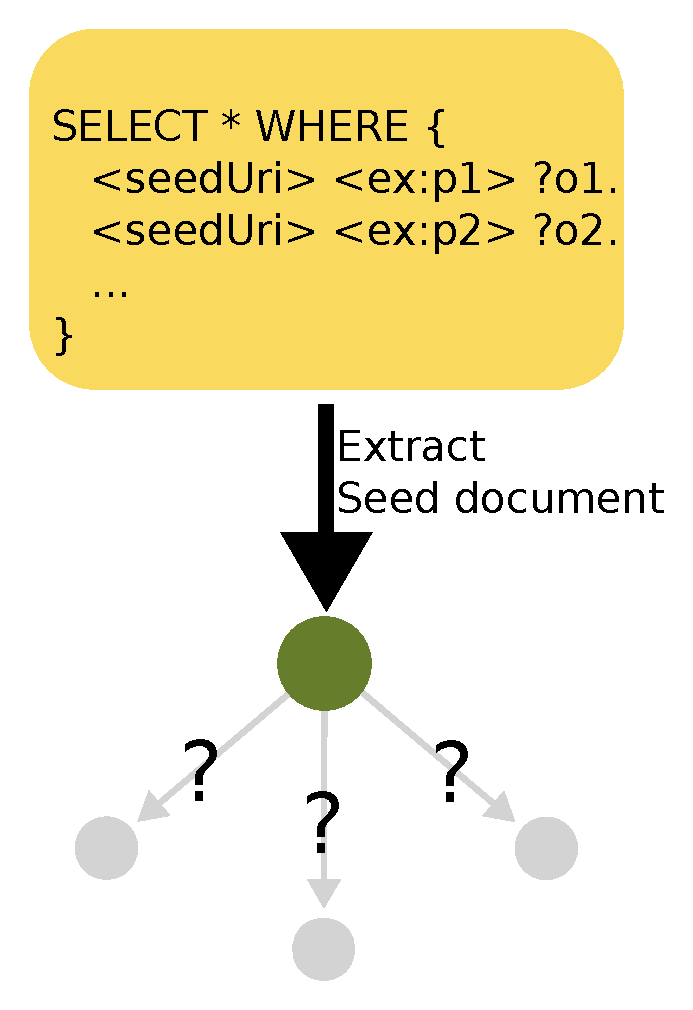
\includegraphics[width=.60\linewidth]{images/hardToOptimizeLTQP.pdf} % replace with your image file
        \end{column}

        % Right column: Text
        \begin{column}{0.4\textwidth}
            The query (partly) determines:
            \begin{itemize}
                \item The queried data
                \item The topology of the queried data
                \item The query-relevant documents
            \end{itemize}
            Result: Limited prior knowledge for query optimization
        \end{column}
    \end{columns}
\end{frame}

\begin{frame}{Query Optimization for Link Traversal: Client-side Engines}
    \begin{columns}[T] % T aligns columns at the top
        % Left column: Image
        \begin{column}{0.6\textwidth} % Adjust width as needed
            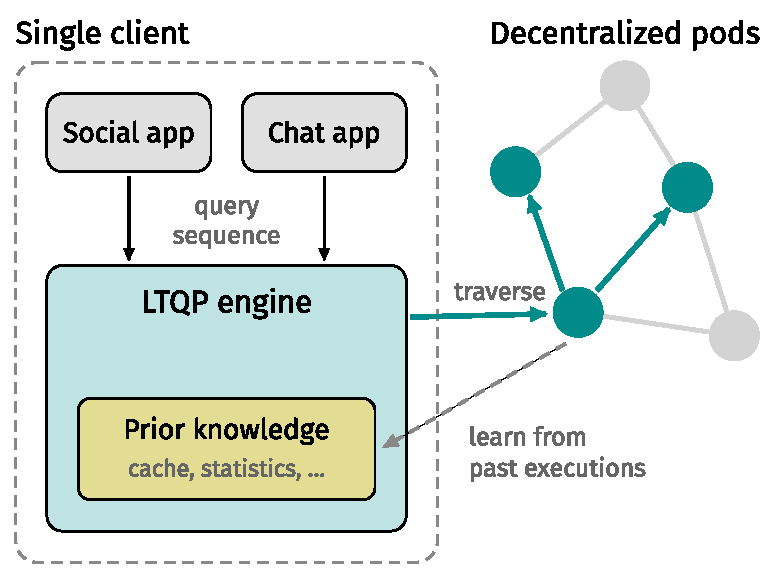
\includegraphics[width=\linewidth]{images/client-side-engine.pdf}
        \end{column}

        % Right column: Text
        \begin{column}{0.4\textwidth}
            \begin{itemize}
                \item Engine instances serve a single client
                \item Can we exploit client-specific usage patterns and `personalize' optimization 
                \item Gain prior knowledge by looking at past executions
            \end{itemize}
        \end{column}
    \end{columns}
\end{frame}


